\section{Particle in an infinite potential well}

\subsection{Introduction (H1)}


\subsection{Distribution of the momentum values in a stationary state}
We have seen that the stationary states of the particle correspond to the energies
\begin{align}
    E_n=\frac{n^2\pi^2\hbar^2}{2ma^2}
\end{align}
and to the wave functions
\begin{align}
    \psi_n(x)=\sqrt{\frac{2}{a}}\sin\frac{n\pi x}{a},
\end{align}
where $a$ is the width of the well.

The probability of a measurement of the momentum $P$ of the particle yielding a result between $p$ and $p+dp$ is
\begin{align}
    \bar{P}_n(p)\;dp=|\bar{\varphi}_n(p)|^2\;dp,\quad\text{with}
\end{align}
\begin{align}
    \bar{\varphi}_n(p)&=\frac{1}{\sqrt{2\pi\hbar}}\int_0^a\sqrt{\frac{2}{a}}\sin\frac{n\pi x}{a}e^{-ipx/\hbar}\;dx\notag\\
    &=\frac{1}{2i\sqrt{n\hbar a}}\int_0^a\left[e^{(\frac{n\pi}{a}-\frac{p}{\hbar})x}-e^{-i(\frac{n\pi}{a}+\frac{p}{\hbar})x}\right]\;dx\label{eq:insidebrackets}\\
    &=\frac{1}{2i}\sqrt{\frac{a}{\pi\hbar}}e^{i(\frac{n\pi}{a}-\frac{pa}{2\hbar})}\left[F(p-\frac{n\pi\hbar}{a})+(-1)^{n+1}F(p+\frac{n\pi\hbar}{a})\right],\quad\text{with}\quad F(p)=\frac{\sin(pa/2\hbar)}{pa/2\hbar}.\notag
\end{align}
The function inside the brakets in equation \eqref{eq:insidebrackets} is even if $n$ is odd, and odd if $n$ is even. The probability density $\bar{P}_n(p)$ is therefore an even function of $p$ in all cases, so that
\begin{align}
    \text{Mean value of the momentum in the energy state $E_n$}\qquad\braket{P}_n=\int_{-\infty}^\infty\bar{P}_n(p)p\;dp=0.
\end{align}
In the same way, we can compute $\braket{P^2}_n$. Using the fact that in the $\{\ket{x}\}$ representation $P$ acts like $-i\hbar\partial_x$ and performing an integration by parts,
we obtain:
\begin{align}
    \braket{P^2}_n=\hbar^2\int_0^a\left|\frac{d\varphi_n}{dx}\right|^2\;dx=\hbar^2\int_0^a\frac{2}{a}\left(\frac{n\pi}{a}\right)^2\cos^2\frac{n\pi x}{a}\;dx=\left(\frac{n\pi x}{a}\right)^2.
\end{align}
Using both $\braket{P}_n$ and $\braket{P^2}_n$ we get:
\begin{align*}
    \Delta P_n=\sqrt{\braket{P^2}_n-\braket{P}_n^2}=\frac{n\pi\hbar}{a}.
\end{align*}

We can plot the probability density $\bar{P}_n(p)$ for different values of $n\in\{1,2,\text{large}\}$. The resutls are illustrated in the followign plot.
\begin{figure}[h!]
    \centering
    \begin{subfigure}{.3\columnwidth}
        \centering
        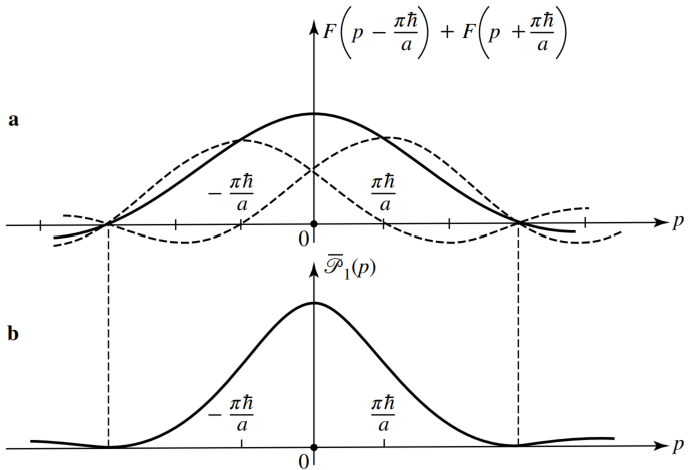
\includegraphics[width=\columnwidth]{PartOne/ChapterTwo/infinitewell_groundstate.png}
        \caption{Ground state ($n=1$)}
    \end{subfigure}
    \hfill
    \begin{subfigure}{.3\columnwidth}
        \centering
        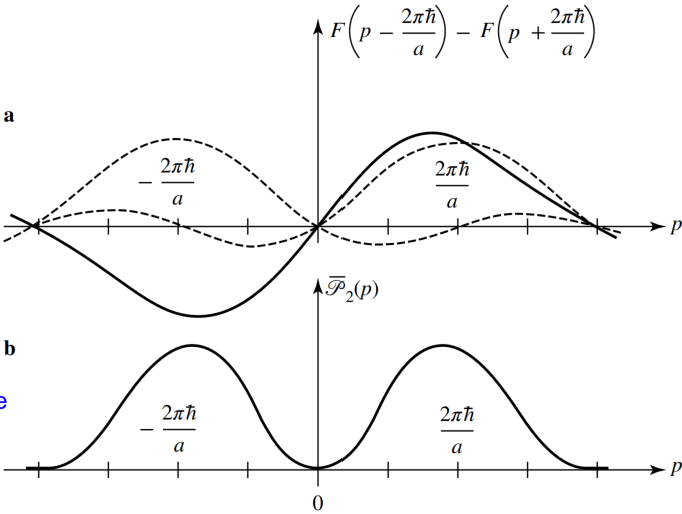
\includegraphics[width=\columnwidth]{PartOne/ChapterTwo/infinitewell_firstexcitedstate.png}
        \caption{First excited state ($n=2$)}
    \end{subfigure}
    \hfill
    \begin{subfigure}{.3\columnwidth}
        \centering
        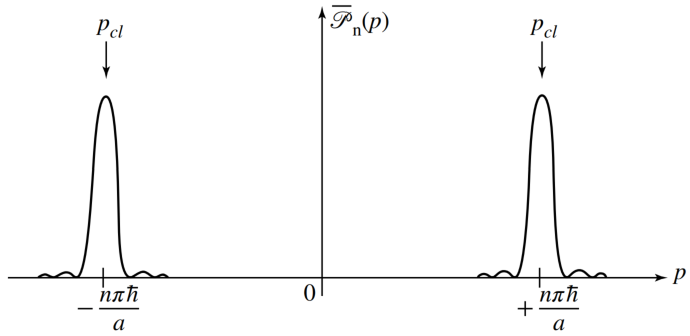
\includegraphics[width=\columnwidth]{PartOne/ChapterTwo/infinitewell_largen.png}
        \caption{State for large $n$}
    \end{subfigure}
\end{figure} 
We can see that as $n$ increase, the interference term between $F(p-n\pi\hbar/a)$ and $F(p+n\pi\hbar/a)$ is negligible:
\begin{align*}
    \bar{P}_n(p)=\frac{a}{4\pi\hbar}\left[F\left(p-\frac{n\pi\hbar}{a}\right)+(-1)^{n+1}F\left(p+\frac{n\pi\hbar}{2}\right)\right]^2\approx\frac{a}{4\pi\hbar}\left[F^2\left(p-\frac{n\pi\hbar}{a}\right)+F^2\left(p+\frac{n\pi\hbar}{a}\right)\right].
\end{align*}
In this limit, is then possible to predict with almost complete certainty the results of a meqasurement of the momentum of the particle in the state $\ket{\varphi_n}$: the value will be nearly equalt to 
$\pm\frac{n\pi\hbar}{a}$, with accuraccy increasing as $n$ grows.
\begin{itemize}[itemsep=0pt,topsep=0pt]
    \item The momentum of a classical particle of energy $E_n$ is:
    \begin{align*}
        \frac{p^2_{cl}}{2m}=\frac{n^2\pi^2\hbar^2}{2ma^2}\longrightarrow p_{cl}=\pm\frac{n\pi\hbar}{a}.
    \end{align*}
    When $n$ is large, the two peaks of $\bar{P}_n(p)$ therefore correspond to the classical values of the momentum.
    \item For large $n$, although the absolute value of the momentum is well-defined, its sign is not. This is why $\Delta P_n$ is large: the rms deviation reflects the distance 
    between the two peaks, it is no longer related to their widths.
\end{itemize}
%%
\subsection{Evolution of the particle's wave function}
Time evolution appears only when the state vector is a inear combination of several kets $\ket{\varphi_n}$. 
%
\subsubsection{Wave function at $t$}
Assuming that at $t=0$ we have 
\begin{align*}
    \ket{\psi(0)}=\frac{1}{\sqrt{2}}[\ket{\varphi_1}+\ket{\varphi_2}],
\end{align*}
we apply formula of this chapter to get 
\begin{align*}
    \ket{\psi(t)}=\frac{1}{\sqrt{2}}\left[e^{-i\frac{\pi^2\hbar}{2ma^2}}\ket{\varphi_1}+e^{-2i\frac{\pi^2\hbar}{ma^2}}\ket{\varphi_2}\right]\propto\frac{1}{\sqrt{2}}[\ket{\varphi_1}+e^{-i\omega_{21}t}\ket{\varphi_2}],\quad\text{with}\quad\omega_{21}=\frac{E_2-E_1}{\hbar}=\frac{3\pi^2\hbar}{2ma^2}.
\end{align*}
%
\subsubsection{Evolution of the shape of the wave packet}
The shape of the wave packet is given by the probability density:
\begin{align*}
    |\psi(x,t)|^2=\frac{1}{2}\varphi_1^2(x)+\frac{1}{2}\varphi_2^2(x)+\varphi_1(x)\varphi_2(x)\cos\omega_{21}t.
\end{align*}
We see that the time variation is due to the interference term in $\varphi_1\varphi_2$. Only one Bohr frequency appears, $\nu_{21}=(E_2-E_1)/\hbar$.

%
\subsubsection{Motion of the center of the wave packet}
The mean value $\braket{X}$ of the position of the particle at $t$ is done by first doing $X'=X-a/2$. By Symmetry, the diagonal matrix elements of $X'$ are zero:
\begin{align*}
    \braket{\varphi_1|X'|\varphi_2}\propto\int_0^a\left(x-\frac{a}{2}\right)\sin^2\frac{\pi x}{a}\;dx=0,\quad\text{and}\quad\braket{\varphi_2|X'|\varphi_2}\propto\int_0^a\left(x-\frac{a}{2}\right)\sin^2\frac{2\pi x}{a}\;dx=0.
\end{align*}
We then have 
\begin{align*}
    \braket{X'}(t)=\re{e^{-i\omega_{21}t}\braket{\varphi_1|X'|\varphi_2}},
\end{align*}
with 
\begin{align*}
    \braket{\varphi_1|X'|\varphi_2}=\braket{\varphi_1|X|\varphi_2}-\frac{a}{2}\braket{\varphi_1|\varphi_2}=\frac{2}{a}\int_0^ax\sin\frac{\pi x}{a}\sin\frac{2\pi x}{a}\;dx=-\frac{16a}{9\pi^2}.
\end{align*}
Therefore, 
\begin{align*}
    \braket{X}(t)=\frac{a}{2}-\frac{16a}{9\pi^2}\cos\omega_{21}t.
\end{align*}
\begin{figure}[h!]
    \centering
    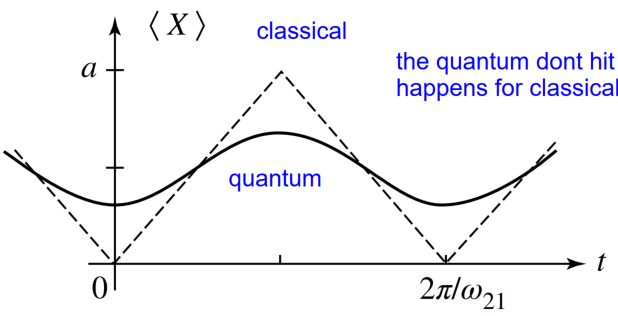
\includegraphics[width=.5\columnwidth]{PartOne/ChapterTwo/meanvalueinfinitewell.png}
    \caption{Time variation of $\braket{X}$ corresponding to the wave packet's motion. QM predicts that the center of the wave packet will turn back before hitting the wall}
\end{figure}
We immediately notice a very clear difference between these two typoe of motion. Before the center of the wave packet has touched the wall, the action of the potential on the edges 
of this packet is sufficient to make it turn back.
\begin{itemize}[itemsep=0pt,topsep=0pt]
    \item The mean value of the energy of the particle in $\ket{\psi(t)}$ is 
    \begin{align*}
        \braket{H}&=\frac{1}{2}E_1+\frac{1}{2}E_2=\frac{5}{2}E_1\\
        \braket{H^2}^=\frac{1}{2}E_1^2+\frac{1}{2}E_2^2=\frac{17}{2}E_1^2,
    \end{align*}
    which gives 
    \begin{align*}
        \Delta H=\frac{3}{2}H_1.
    \end{align*}
    We have seen that the wave packet evolves appreciably over a time of the order of $\Delta t\approx1/\omega_{21}$. Therefore,
    \begin{align}
        \Delta H\Delta t=\frac{3}{2}E_1\frac{\hbar}{3E_1}=\frac{\hbar}{2}.
    \end{align}
\end{itemize}

\subsection{Perturbation created by a position measurement}